\documentclass[10pt,aspectratio=169]{beamer}
\usetheme{default}\usecolortheme{seagull}\setbeamertemplate{navigation symbols}{}
\setbeamertemplate{footline}{\hfill\scriptsize\insertframenumber/\inserttotalframenumber\hspace{2mm}\vspace{1mm}}
\usepackage{booktabs,graphicx,amsmath}
\graphicspath{{../report/figures/}}
\title{Lost in Pooling: Recovering Small-Signal Evidence Discarded by Frozen Foundation Models}
\subtitle{CSCI 566 project clinic}
\author{Dhairya Shah \and Raghav Sarmukaddam \and Yash Desai \and Prisha Thakur \and Ansh Parasher \and Advait Kale}
\institute{University of Southern California}
\date{November 23, 2026}
\begin{document}
\frame{\titlepage}

\begin{frame}{The question}
\begin{itemize}
\item Frozen ViT backbones are deployed as \textbf{one pooled vector} per image (CLS or mean of patch tokens) plus a linear probe.
\item A recent chest X-ray study found CLS probes at chance on small lesions while the same models' patch tokens, restricted to the lesion, kept the signal.
\item \textbf{Hypothesis:} the evidence survives the encoder and is lost at \emph{aggregation}.
\item \textbf{Test:} on identical cached tokens, swap only the read-out: CLS, mean, max, an oracle that pools the ground-truth region, a max-MIL head and a gated attention head trained from image-level labels only.
\item \textbf{Measure:} per-class AUROC stratified by the relative size of the largest instance (the \emph{blindness curve}).
\end{itemize}
\end{frame}

\begin{frame}{Pre-proposal feedback and what we did with it}
\begin{columns}
\column{0.5\textwidth}
\textbf{Feedback}
\begin{itemize}
\item Scope: one dataset and one backbone first.
\item Causal claim: cross-modal similarity is not cause; use the controlled pooling swap.
\item Keep negative findings specific.
\item Audio and distillation wait.
\end{itemize}
\column{0.5\textwidth}
\textbf{Done}
\begin{itemize}
\item MS-COCO 2017 + DINOv2 ViT-B/14 first; then CLIP, SigLIP, DINO ViT-B/16.
\item Every read-out on the same tokens; oracle vs global on the same images.
\item NIH ChestX-ray14 (+ RAD-DINO, 448 px, ChestX-Det10 in progress).
\item Distillation and LUNA16 scheduled last.
\end{itemize}
\end{columns}
\end{frame}

\begin{frame}{Blindness curve, COCO val2017, DINOv2 ViT-B/14 at 224 px}
\centering
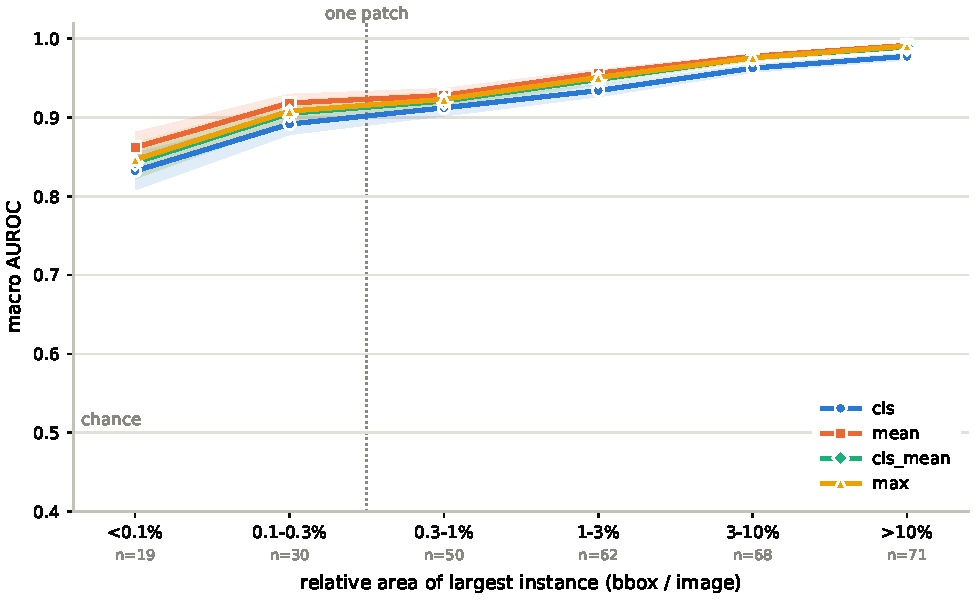
\includegraphics[width=0.62\textwidth]{blindness_curve__dinov2_vitb14_reg__res224.pdf}
\begin{itemize}\small
\item Global read-outs fall from 0.99 AUROC on large targets to 0.84--0.86 on sub-patch targets ($<0.1\%$ of the image).
\item The oracle, pooling only the ground-truth region of the \emph{same} tokens, stays at 0.97: the loss is at pooling.
\item The attention head (no boxes) reaches 0.89 ($0.90$ multi-scale); mAP 0.73 $\rightarrow$ 0.80 (0.82).
\end{itemize}
\end{frame}

\begin{frame}{Same pattern on four backbones}
\centering
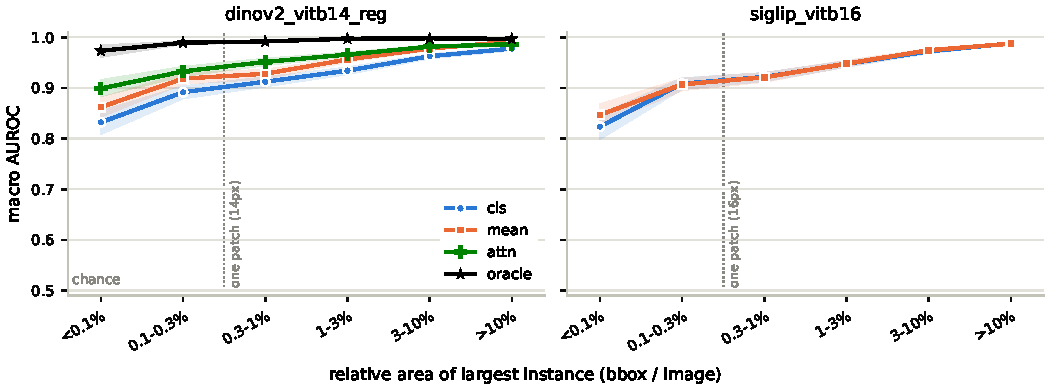
\includegraphics[width=0.95\textwidth]{cross_backbone__res224.pdf}
\begin{itemize}\small
\item DINOv2, CLIP ViT-B/16, SigLIP ViT-B/16, DINO ViT-B/16: global read-outs 0.80--0.86 on sub-patch targets, oracles 0.90--0.97, heads in between on each.
\item DINO ViT-B/16 (self-supervised, 16 px) has the weakest tokens: patch size does not decide how much small-object evidence survives the encoder; the pretraining recipe does.
\item Three seeds per head; paired bootstrap intervals exclude zero in the small bins.
\end{itemize}
\end{frame}

\begin{frame}{Where does the head look?}
\centering
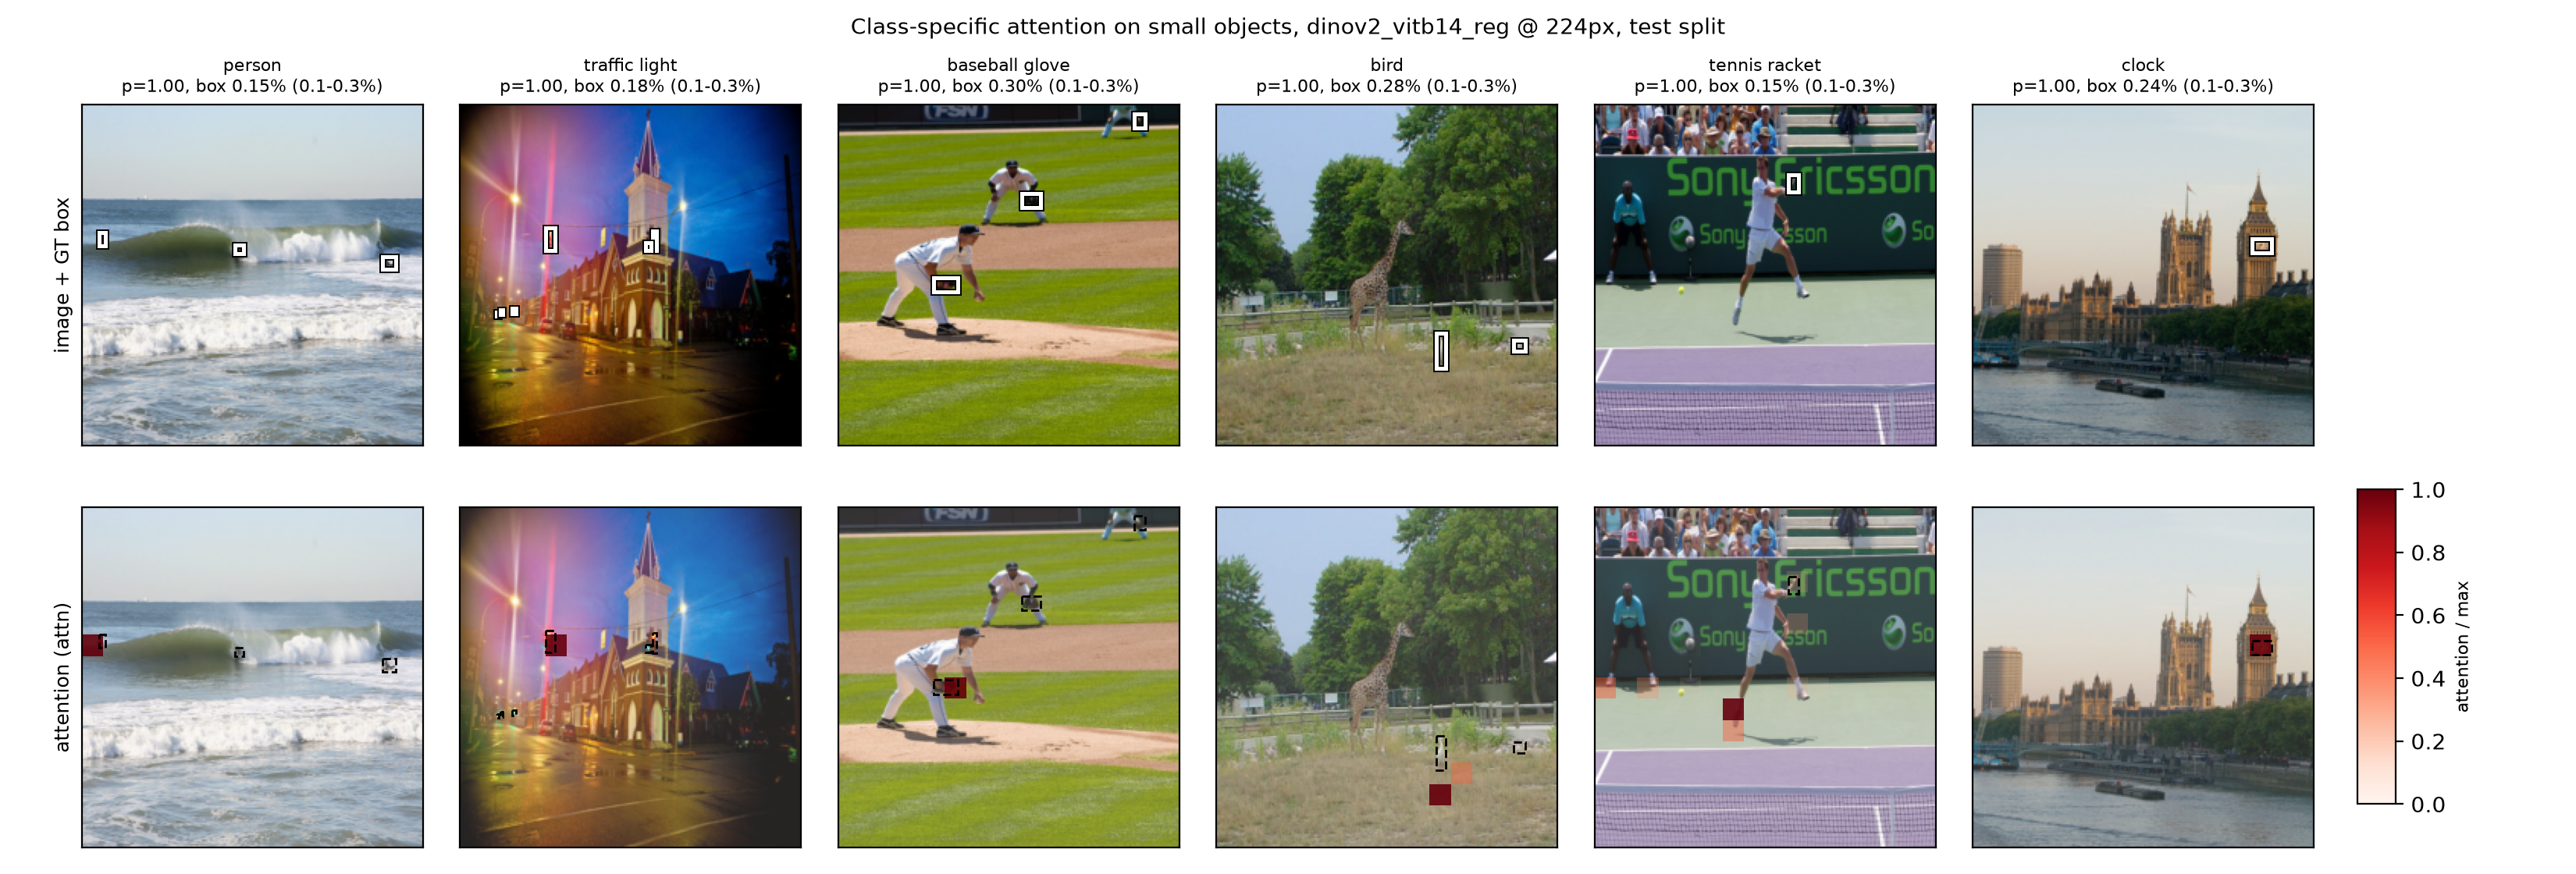
\includegraphics[width=0.9\textwidth]{attention_examples.png}
\begin{itemize}\small
\item Attention mass inside the ground-truth box is 12 to 24 times chance on small targets; the head learned the object, not only its context.
\item Classes that global pooling loses are the ones with unpredictable scenes (banana, motorcycle); the per-class oracle gap tracks a context score (Spearman $-0.98$).
\item \textbf{Context-only control:} pooling only the tokens \emph{outside} the box scores 0.862 on sub-patch targets, the mean probe's 0.862 exactly. On a sub-patch target a global read-out does no better than one forbidden to see the target.
\end{itemize}
\end{frame}

\begin{frame}{Mechanism: token fraction vs patches covered}
\centering
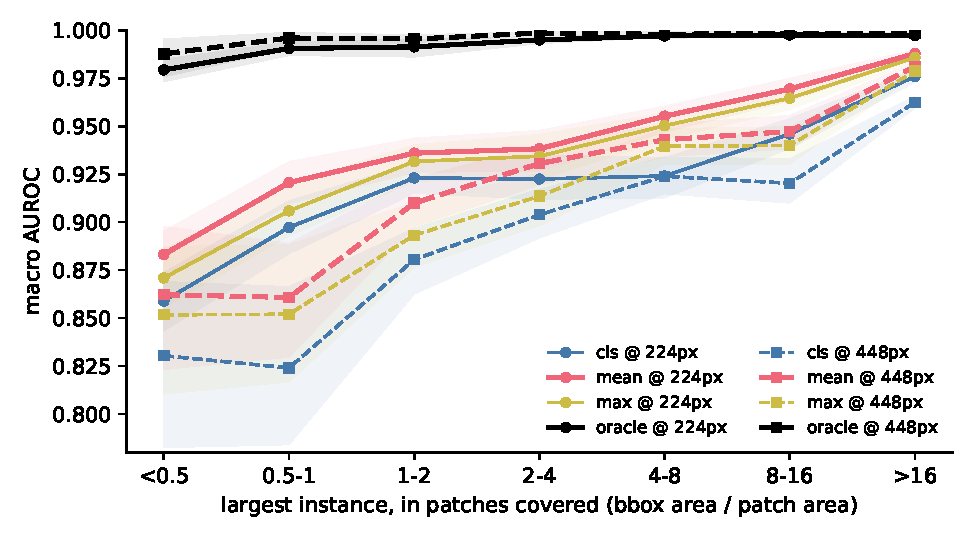
\includegraphics[width=0.8\textwidth]{patch_units__dinov2_vitb14_reg.pdf}
\begin{itemize}\small
\item 224, 336 and 448 px on the same images. The oracle's curves coincide in \emph{patch} units: more pixels per object help a region read-out.
\item Global pooling orders itself by \emph{token fraction}: at 448 px a small object is the same share of four times as many tokens, and the probe does not improve.
\end{itemize}
\end{frame}

\begin{frame}{Radiographs: the cliff reappears (NIH ChestX-ray14, 880 boxed images)}
\begin{columns}
\column{0.5\textwidth}
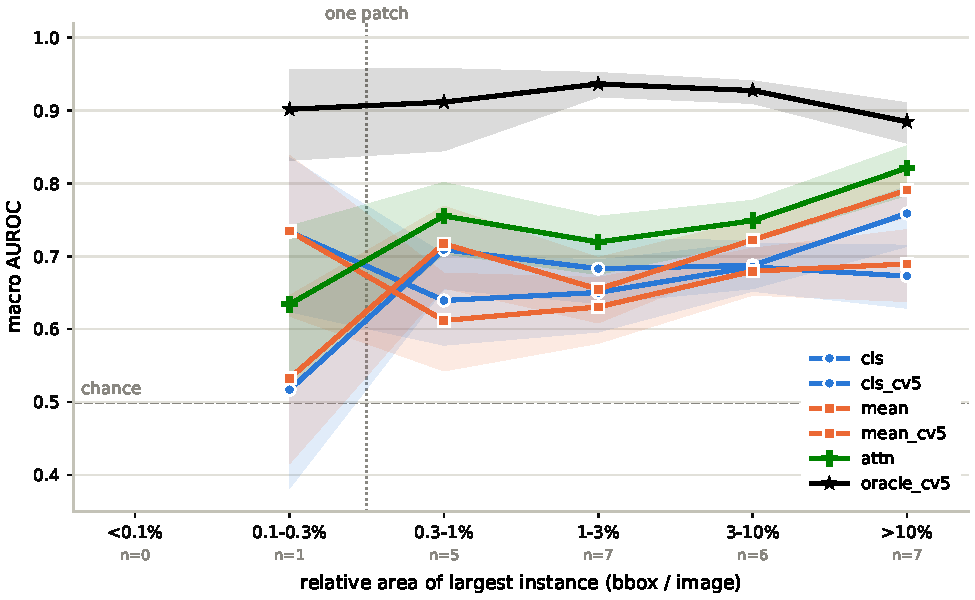
\includegraphics[width=\textwidth]{blindness_curve__dinov2_vitb14_reg__res224_cxr.pdf}
\column{0.5\textwidth}\small
{\scriptsize\begin{tabular}{@{}lcc@{}}\toprule
DINOv2, 224 px & global & oracle \\ \midrule
5-fold CV, boxed images & 0.58 & 0.88--0.94 \\
image-level training (20,721) & 0.70 & -- \\
attention head (3 seeds) & $0.73\pm0.02$ & -- \\ \bottomrule
\end{tabular}}
\begin{itemize}
\item No scene prior: every radiograph is a chest, so the pooled vector has nothing to fall back on.
\item RAD-DINO (radiograph-adapted) raises both sides (oracle 0.95--0.97, probes 0.77) without closing the gap.
\item At 448 px on the full cache the head gains 0.04 ($0.77\pm0.01$), the global probes 0.01--0.02. RAD-DINO at 448 px: head $0.80\pm0.01$ vs.\ mean probe 0.81 overall, but the head leads in every size bin ($+0.12$ at 0.1--0.3\%).
\item ChestX-Det10 (3,543 images, 10 findings, 5.4$\times$ the boxes): same cliff (global 0.56--0.69 vs oracle 0.91--0.93 under 0.3\%); NIH-trained head transfers: 0.74 vs 0.69 (CLS) at 224 px, 0.77 vs 0.70 at 448 px; RAD-DINO 0.83 vs 0.80.
\end{itemize}
\end{columns}
\end{frame}

\begin{frame}{Tiled-teacher distillation: a negative result}
NIH radiographs, DINOv2, three seeds, macro AUROC (0.1--0.3\% lesions / all)
\begin{center}\small\begin{tabular}{@{}lcc@{}}\toprule
Read-out (tokens at test time) & 0.1--0.3\% & All \\ \midrule
224 px head, baseline (224 px) & $0.61\pm0.04$ & $0.73\pm0.02$ \\
Inference-time tiling, $4\times$ compute (448 px) & 0.58 & 0.73 \\
448 px head, teacher (448 px) & $\mathbf{0.72\pm0.01}$ & $\mathbf{0.77\pm0.01}$ \\
Student of the tiled teacher (224 px) & $0.58\pm0.03$ & $0.74\pm0.02$ \\
Student of the 448 px teacher (224 px) & $0.63\pm0.05$ & $0.72\pm0.01$ \\ \bottomrule
\end{tabular}\end{center}
\begin{itemize}\small
\item Neither student moves off the baseline in any bin; tiling at test time does not either.
\item The 448 px head's extra evidence is not in the 224 px tokens: it was lost at patch embedding, and a teacher cannot supply what the student's input does not contain.
\item Resolution gains on small findings must be bought at the encoder's input. % TODO(final): COCO
\end{itemize}
\end{frame}

\begin{frame}{A pre-deployment check}
\centering
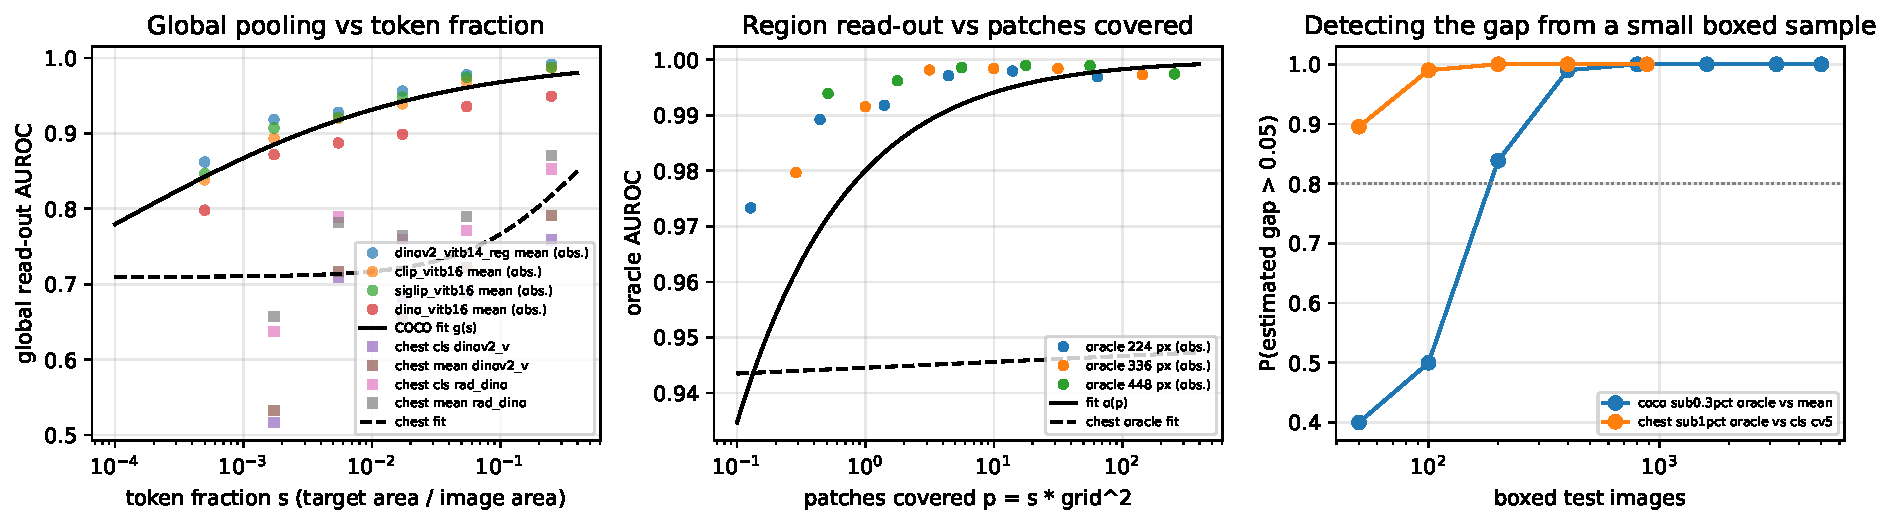
\includegraphics[width=0.98\textwidth]{deploy_check.pdf}
\begin{itemize}\small
\item Global AUROC as a logistic function of token fraction: within 0.02 across resolutions, leave-one-backbone-out error $\le 0.012$; the radiograph offset (0.17--0.28) is the missing scene prior.
\item Oracle AUROC as a function of patches covered. Given a target size and a token grid, the two curves predict the loss.
\item 200 boxed images detect the sub-patch gap on COCO with power 0.84; 50 suffice on radiographs.
\end{itemize}
\end{frame}

\begin{frame}{What we would like feedback on}
\begin{enumerate}
\item \textbf{The causal argument.} Same tokens, swap the read-out: is the oracle-vs-global comparison plus the resolution mechanism test enough, or should we add an intervention (e.g. masking tokens outside the box for the global probe)?
\item \textbf{Context priors.} The context-only control now shows the floor of the global read-outs is the scene. Is that control convincing, or should we also mask tokens inside the box for the global probe at training time?
\item \textbf{Extensions.} ChestX-Det10, DINO ViT-B/16 and distillation (negative) are in; the scoped LUNA16 slice arm is running. Is the negative distillation result worth a section of its own?
\item \textbf{Framing.} Is the blindness curve plus the deployment check the right headline for the final report?
\end{enumerate}
\end{frame}

\begin{frame}{Plan to the final report (Dec 7)}
\begin{tabular}{p{0.2\textwidth}p{0.75\textwidth}}\toprule
Nov 23--29 & Finish ChestX-Det10, DINO ViT-B/16, seeds for every read-out, distillation; poster. \\
Nov 30 & Poster and live demo: blindness curve and attention maps on a user-chosen image. \\
Nov 30--Dec 6 & LUNA16 slice arm; consolidate; final report in the midterm format. \\
Dec 7 & Final report, released code, cached curves and reproduction commands. \\ \bottomrule
\end{tabular}
\vspace{4mm}

Code and results: \texttt{github.com/DhairyaShah5/lost-in-pooling}
\end{frame}
\end{document}
